\documentclass[a4paper,12pt]{article}
\usepackage{graphicx}
\usepackage{fancyhdr}
\pagestyle{fancy}
\rhead{Dane Johnson}
\title{CS-456 Project 1}
\author{Dane Johnson}
\date{February 7th, 2018}
\headheight=15pt
\begin{document}
\maketitle
\newpage
\section{Motivation}

The motivation for this project is to use Quicksort and Mergesort algorithms to practice empirical analysis of algorithms.
This includes creating diagrams and statistics to prove my implementation of the algorithms is correct.

Additionally, this project will serve as an exercise in writing pseudocode, proving its correctness and using invariants.
\section{Algorithms}
\subsection{Quicksort}
\subsubsection{Pseudocode}
\begin{verbatim}
proc quicksort(A, start, end)
  if start < end
    pivot <- A[end]
    i <- start - 1 
    for j <- start to end - 1
      if A[j] < pivot
        i++
        swap A[i] and A[j]
    if A[end] < A[i + 1]
      swap A[end] and A[i + 1]
    quicksort(A, start, i)
    quicksort(A, i + 2, end)
\end{verbatim}
\subsubsection{Correctness Proof}
\begin{description}
\item [Invariant: ] Given $k$, a number between $start$ and $end$
  \begin{enumerate}
  \item If $start \leq k \leq i$ then $A[k] \leq pivot$
  \item If $i + 1 \leq k \leq j - 1$ then $A[k] > pivot$
  \item If $k = end$ then $A[k] = pivot$
  \end{enumerate}
\item [Initialization: ] Before the first loop, $start$ and $end$ are the same, so no values
  lie in this range. Therefore the only $k$ that may be chosen id $end$, which is trivially
  equivalent to $pivot$.
\item [Maintenence: ] Two cases exist.
  \begin{enumerate}
  \item If $A[j] > pivot$, we merely increment $j$, and the second condition holds for $A[j - 1]$ and all other
    entries are unchanged.
  \item If $A[j] \leq pivot$, $A[i]$ is swapped with $A[j]$. Incrementing $j$ then gives $A[i] < pivot$, which satifies
    the first condition.
  \end{enumerate}
\item [Termination: ] When the loop terminates $j = end$, and all values of the array now fall into one of the three
  conditions of the invariant.
\end{description}
\subsection{Quicksort (Array)}
\subsubsection{Issues}
Quicksort as an array is easy enough to implement. Main problem would be assuring the list is partititioned correctly.
\subsubsection{Benchmark Data}
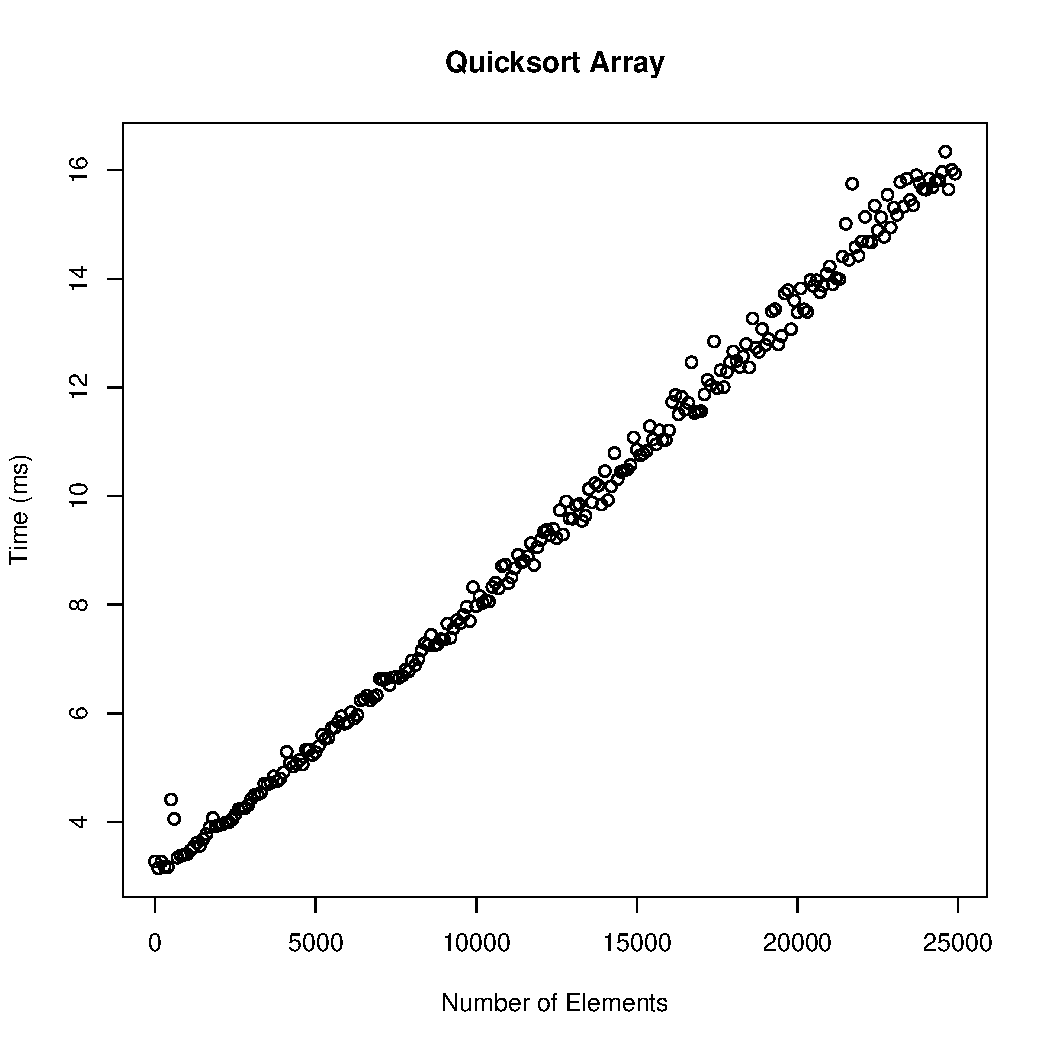
\includegraphics[height=10cm]{quicksort_array}
\subsubsection{Observations}
Quicksort behaves as expected. $O(nlg(n))$, which is best case for any sort, and is clearly seen in the data.
$n$ iterations comes from the list being subdivided, ultimately, into $n$ lists. $lg(n)$ comes from partitioning the list, which
halves in size each recursive call.
\subsection{Quicksort (Linked List)}
\subsubsection{Issues}
A lot of issues crop up with Quicksorting a list. Without random access abilites, partitioning the list becomes a chore
involving ensuring a pointer moving up the list remains before the tail value. A little bit of fudge is necessary to
terminate before the incrementing pointer moves past the end of the sublist.
\subsubsection{Benchmark Data}
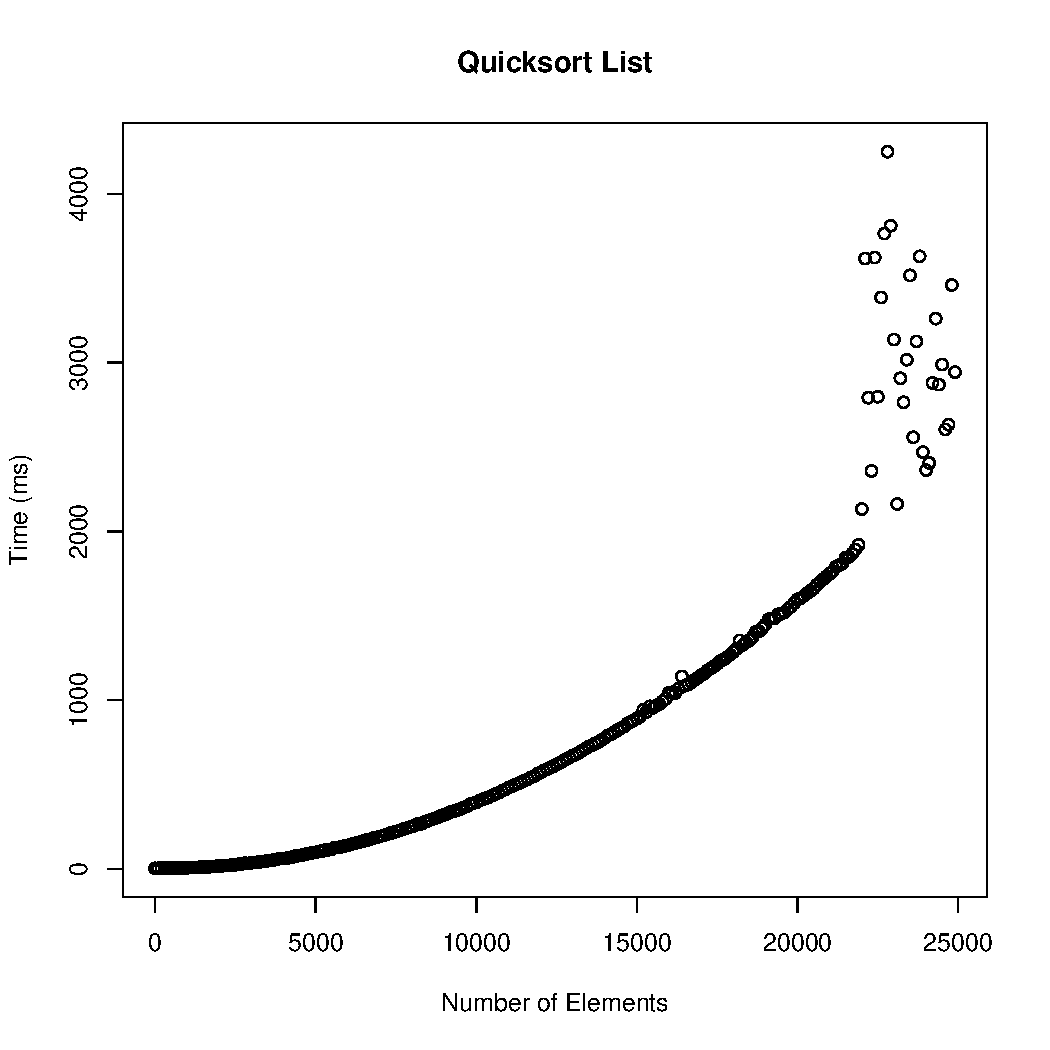
\includegraphics[height=10cm]{quicksort_list}
\subsubsection{Observations}
After careful consideration, I have come to believe that the data returned from the benchmark does follow the expected $O(nlg(n))$
complexity. The question remains as to why it is so much slower than the other algorithms. I think this is due to how much stack space is devoted to
pointer arithmetic, and the fact that this memory was not freed at any point in the benchmark.
\subsection{Mergesort}
\subsubsection{Pseudocode}
\begin{verbatim}
proc mergesort(A)
  if A.length > 1
    divide A into A1 and A2
    mergesort(A1)
    mergesort(A2)
    merge(A1, A2, A)
proc merge(A1, A2, A)
  i <- 0
  j <- 0
  while i < A1.length or j < A2.length
    if i = A1.length
      A[i + j] <- A2[j]
      j++
    else if j = A2.length
      A[i + j] <- A1[i]
      i++
    else if A1[i] > A2[j]
      A[i + j] <- A1[i]
      i++
    else 
      A[i + j] <- A2[j]
      j++     
\end{verbatim}
\subsubsection{Correctness Proof}
\begin{description}
\item [Invariant: ] At the beginning of each iteration, $A1$ and $A2$ are sorted, $A$ contains the $i + j$ smallest elements
  from $A1$ and $A2$ and $A1[i]$ and $A1[j]$ are the smallest values in their respective arrays that have not been copied into $A$.
\item [Initilization: ] Initially $A[i]$ and $A[j]$ are both the first and therefore smallest values in thier respective arrays, and nothing has been
  copied into $A$, so it is trivially sorted.
\item [Maintenence: ] If $j = A2.length$ or $A1[i] < A2[i]$, then $i$ is the smallest value that has not been copied into $A$ and copying it into
  $A$ means $A$ contains $i + j + 1$ sorted elements. This is true for $j$ in the cases where $i = A2.length$ or $A1[i] \geq A2[j]$.
\item [Termination: ] When the loop completes, $i + j$ is the length of the two subarrays, which is the length of $A$. This impies that the entire array is sorted.
\end{description}
\subsection{Mergesort (Array)}
\subsubsection{Issues}
Again, no real issues implementing mergesort. I did hit a snag where I was overstepping the bounds of my array, but I added extra cases for them. Having
now read the section in the book, I realized that an infinite sentinel value and a \texttt{for} loop could also have sufficed.
\subsubsection{Benchmark Data}
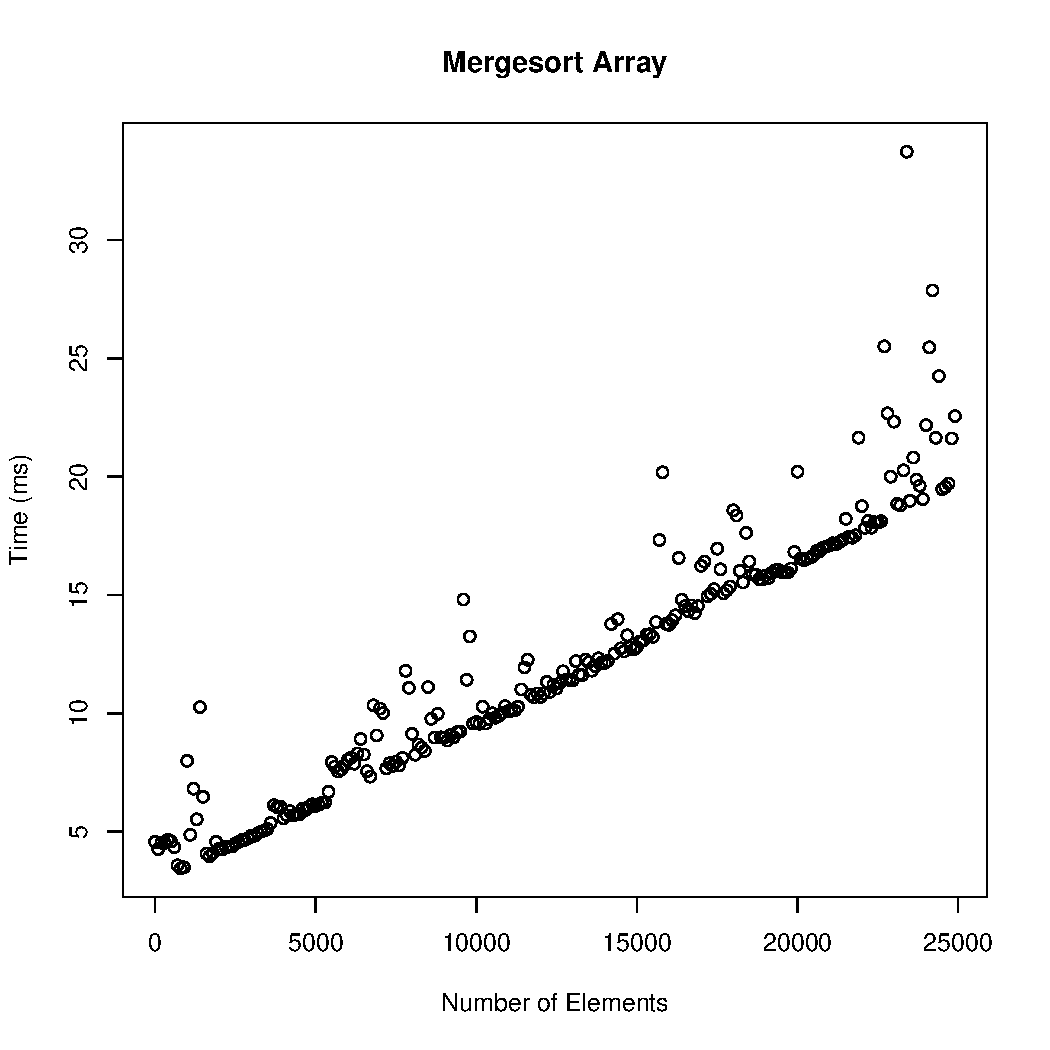
\includegraphics[height=10cm]{mergesort_array}
\subsubsection{Observations}
The data here seems to closely follow the expected runtime of $O(nlg(n))$. There are a few outliers near powers of two, but I expect those come from the computer's needing
to free up memory to hold the additional stack space. The runtime complexity comes from merging $n$ arrays $lg(n)$ times to recreate the original array in sorted form.
\subsection{Mergesort (Linked List)}
\subsubsection{Issues}
Splitting and combining linked lists requires a bit more attention than an array does, but ultimately when given consideration is not that much more difficult.
\subsubsection{Benchmark Data}
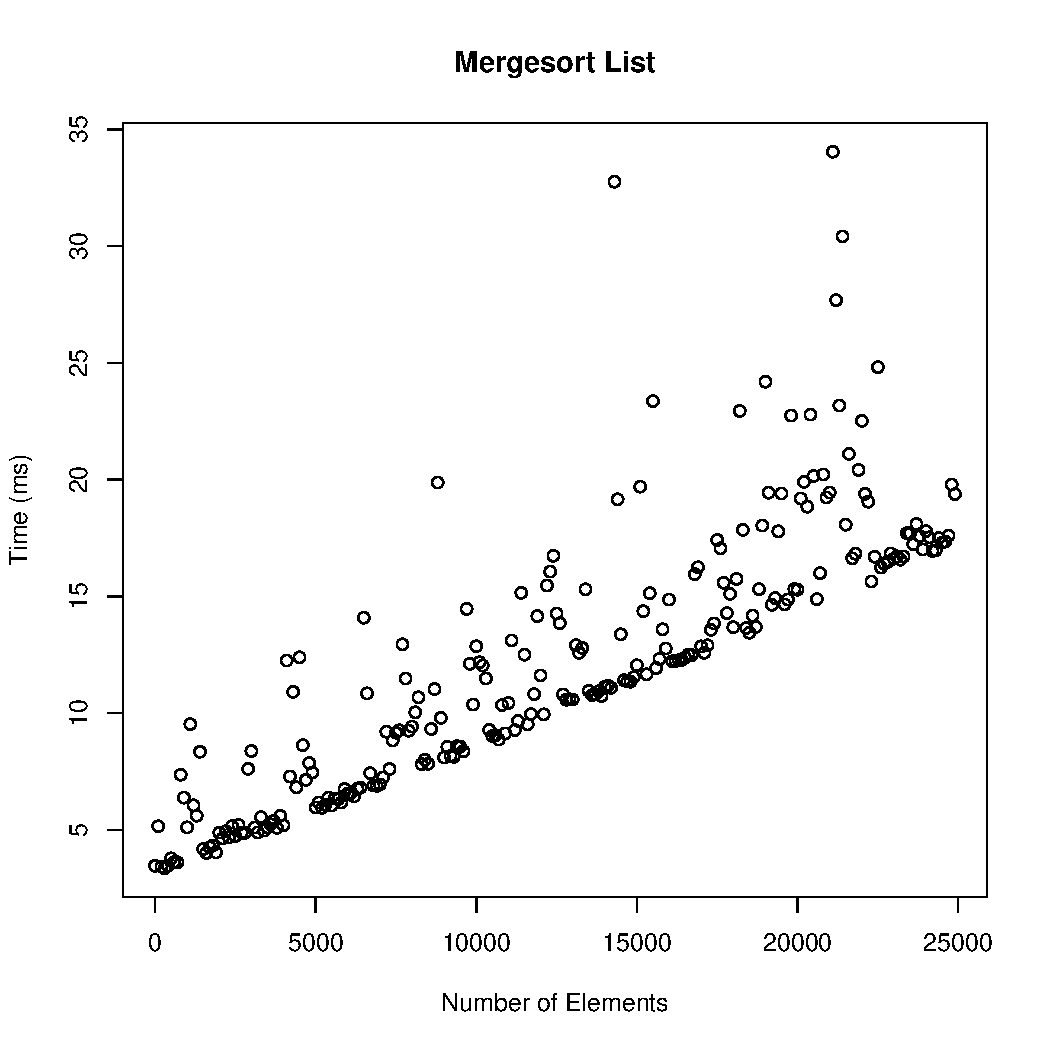
\includegraphics[height=10cm]{mergesort_list}
\subsubsection{Observations}
The data again seems to follow the expected runtime. There are a few more outliers in this implementation, but I am convinced that they are caused the same way as
the arrays, just with greater extremes as a result of needing to pull stack space off the heap.
\section{Conclusion}
All in all, these sorts all have the same asymptotic time complexity given a random input series. In this average case, selecting quicksort or mergesort for an
array comes down to a matter of taste. Quicksort, while somewhat less readable, uses less space than a mergesort, and provided the system has RAM enough, it should
not be an issue. Quicksorting a list has proven to have significant overhead cost that mergesort would not present, so I would outright suggest the mergesort on a list.

In the worst case, mergesort is the clear victor. Mergesort has no varience in execution based on input, besides which subarray is completed merging first.
Mergesort therefore has a tight-bound, $\Theta(nlg(n))$. Quicksort does not have this property. Quicksort's speed is dependent on the selection of a pivot that comes as close as possible
to bisecting the list. This means that if the list is in a sorted or reverse sorted order, or nearly enough to either, then quicksort is reduced to sorting $n$ sublists $n$ times.
Therefore, while quicksort has $O(nlg(n))$ best case, it has $\Omega(n^2)$ as a worst case. Therefore, if there is a possibility that the input will be sorted or nearly sorted,
mergesort should be selected.

As far as the graphs, apart from the slight variations from the norm described in each section, they all follow the same $nlg(n)$ curve, as they are all run on random data sets.
\end{document}
